\section{مدیریت مراجع در لاتک}\label{App:RefMan}
در بخش \ref{Sec:Ref} اشاره شد که با دستور 
 \lr{\textbackslash bibitem}
  می‌توان یک مرجع را تعریف نمود و با فرمان
 \lr{\textbackslash cite}
  به آن ارجاع داد. این روش برای تعداد مراجع زیاد و تغییرات آنها مناسب نیست. در ادامه به صورت مختصر توضیحی در خصوص برنامه \lr{BibTeX} که همراه با توزیع‌های معروف تِک عرضه می‌شود و نحوه استفاده از آن در زی‌پرشین خواهیم داشت.

\subsection{ مدیریت مراجع با  \texorpdfstring{\lr{Bib\TeX}}{Bib\TeX} }
یکی از روش‌های قدرتمند و انعطاف‌پذیر برای نوشتن مراجع مقالات و مدیریت مراجع در لاتک، استفاده از  \lr{BibTeX} است.
 روش کار با  \lr{BibTeX} به این صورت است که مجموعه‌ی همه‌ی مراجعی را که در پروژه/پایان‌نامه/رساله استفاده کرده یا خواهیم کرد، 
در پرونده‌ی جداگانه‌ای نوشته و به آن فایل در سند خودمان به صورت مناسب لینک می‌دهیم.
 کنفرانس‌ها یا مجله‌های گوناگون برای نوشتن مراجع، قالب‌ها یا قراردادهای متفاوتی دارند که به آنها استیلهای مراجع گفته می‌شود.
 در این حالت به کمک ‌استیل‌های \lr{BibTeX} خواهید توانست تنها با تغییر یک پارامتر در پرونده‌ی ورودی خود، مراجع را مطابق قالب موردنظر تنظیم کنید. 
 بیشتر مجلات و کنفرانس‌های معتبر یک پرونده‌ی سبک (\lr{BibTeX Style}) با پسوند \lr{bst} در وب‌گاه خود می‌گذارند که برای همین منظور طراحی شده است.

به جز نوشتن مقالات این سبک‌ها کمک بسیار خوبی برای تهیه‌ی مستندات علمی همچون پایان‌نامه‌هاست که فرد می‌تواند هر قسمت از کارش را که نوشت مراجع مربوطه را به بانک مراجع خود اضافه نماید. با داشتن چنین بانکی از مراجع، وی خواهد توانست به راحتی یک یا چند ارجاع به مراجع و یا یک یا چند بخش را حذف یا اضافه ‌نماید؛ 
مراجع به صورت خودکار مرتب شده و فقط مراجع ارجاع داده شده در قسمت کتاب‌نامه خواهندآمد. قالب مراجع به صورت یکدست مطابق سبک داده شده بوده و نیازی نیست که کاربر درگیر قالب‌دهی به مراجع باشد. 
در این جا مجموعه‌ سبک‌های بسته \lr{Persian-bib} که برای  زی‌پرشین آماده شده‌اند به صورت مختصر معرفی شده و روش کار با آن‌ها گفته می‌شود. برای اطلاع بیشتر به راهنمای بسته‌ی \lr{Persian-bib} مراجعه فرمایید.
\subsection{سبک‌های فعلی قابل استفاده در زی‌پرشین}
در حال حاضر فایلهای سبک زیر برای استفاده در زی‌پرشین آماده شده‌اند:

\singlespacing
\begin{description}
\item [\lr{unsrt-fa.bst}] این سبک متناظر با \lr{unsrt.bst} می‌باشد. مراجع به ترتیب ارجاع در متن ظاهر می‌شوند.
\item [\lr{plain-fa.bst}] این سبک متناظر با \lr{plain.bst} می‌باشد. مراجع بر اساس نام‌خانوادگی نویسندگان، به ترتیب صعودی مرتب می‌شوند.
 همچنین ابتدا مراجع فارسی و سپس مراجع انگلیسی خواهند آمد.
\item [\lr{acm-fa.bst}] این سبک متناظر با \lr{acm.bst} می‌باشد. شبیه \lr{plain-fa.bst} است.  قالب مراجع کمی متفاوت است. اسامی نویسندگان انگلیسی با حروف بزرگ انگلیسی نمایش داده می‌شوند. (مراجع مرتب می‌شوند)
\item [\lr{ieeetr-fa.bst}] این سبک متناظر با \lr{ieeetr.bst} می‌باشد. (مراجع مرتب نمی‌شوند)
\item [\lr{plainnat-fa.bst}] این سبک متناظر با \lr{plainnat.bst} می‌باشد. نیاز به بسته \lr{natbib} دارد. (مراجع مرتب می‌شوند)
\item [\lr{chicago-fa.bst}] این سبک متناظر با \lr{chicago.bst} می‌باشد. نیاز به بسته \lr{natbib} دارد. (مراجع مرتب می‌شوند)
\item [\lr{asa-fa.bst}] این سبک متناظر با \lr{asa.bst} می‌باشد. نیاز به بسته \lr{natbib} دارد. (مراجع مرتب می‌شوند)
\item[\lr{ModifiedIEEEtranFa.bst}] این سبک متناظر با نحوه ارجاع در پایان‌نامه‌های دانشگاه صنعتی اصفهان می‌باشد.
\end{description}
\doublespacing

با استفاده از استیلهای فوق می‌توانید به انواع مختلفی از مراجع فارسی و لاتین ارجاع دهید. به عنوان نمونه مرجع 
\cite{Omidali82phdThesis}
 یک نمونه پروژه دکترا (به فارسی) و مرجع 
\cite{Vahedi87} یک نمونه مقاله مجله فارسی است.
مرجع 
\cite{Amintoosi87afzayesh}  یک نمونه  مقاله کنفرانس فارسی و
مرجع 
\cite{Pedram80osool} یک نمونه کتاب فارسی با ذکر مترجمان و ویراستاران فارسی است. مرجع 
\cite{Khalighi07MscThesis} یک نمونه پروژه کارشناسی ارشد انگلیسی و
\cite{Khalighi87xepersian} هم یک نمونه متفرقه  می‌باشند.
مراجع 
\cite{Gonzalez02book,Baker02limits} 
نمونه کتاب و مقاله انگلیسی هستند.

استیل مورد استفاده در این پروژه/پایان‌نامه/رساله 
\lr{ModifiedIEEEtranFa}
است که خروجی آنرا در بخش مراجع می‌توانید مشاهده کنید.
نمونه  خروجی سبک \lr{asa-fa} در شکل \ref{fig:asafa} آمده است.

\begin{figure}[t]
\centering
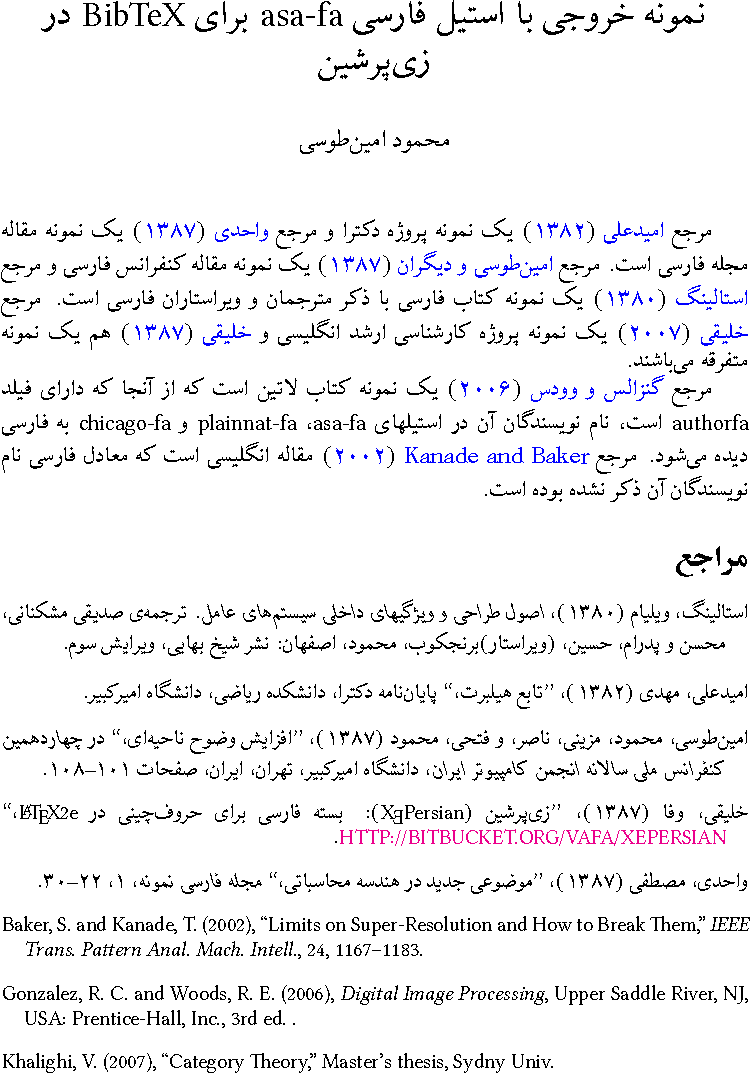
\includegraphics[width=.8\textwidth]{Figures/App1/asa-fa-crop.pdf}
\caption{نمونه خروجی با سبک \lr{asa-fa}}
\label{fig:asafa}
\end{figure} 
\subsection{ نحوه استفاده از سبک‌های فارسی}
برای استفاده از بیب‌تک باید مراجع خود را در یک فایل با پسوند \lr{bib} ذخیره نمایید. یک فایل \lr{bib} در واقع یک پایگاه داده از مراجع\LTRfootnote{Bibliography Database}  شماست که هر مرجع در آن به عنوان یک رکورد از این پایگاه داده
با قالبی خاص ذخیره می‌شود. به هر رکورد یک مدخل\LTRfootnote{Entry} گفته می‌شود. یک نمونه مدخل برای معرفی کتاب \lr{Digital Image Processing} در ادامه آمده است:

\singlespacing
\begin{LTR}
\begin{verbatim}
@BOOK{Gonzalez02image,
  AUTHOR =      {Rafael Gonzalez and Richard Woods},
  TITLE =       {Digital Image Processing},
  PUBLISHER =   {Prentice-Hall, Inc.},
  YEAR =        {2006},
  EDITION =     {3rd},
  ADDRESS =     {Upper Saddle River, NJ, USA}
}
\end{verbatim}
\end{LTR}
\doublespacing

در مثال فوق، \lr{@BOOK} مشخصه‌ی شروع یک مدخل مربوط به یک کتاب و \lr{Gonzalez02book} برچسبی است که به این مرجع منتسب شده است.
 این برچسب بایستی یکتا باشد. برای آنکه فرد به راحتی بتواند برچسب مراجع خود را به خاطر بسپارد و حتی‌الامکان برچسب‌ها متفاوت با هم باشند معمولاً از قوانین خاصی به این منظور استفاده می‌شود. یک قانون می‌تواند فامیل نویسنده‌ی اول+دورقم سال نشر+اولین کلمه‌ی عنوان اثر باشد. به \lr{AUTHOR} و $\dots$ و \lr{ADDRESS} فیلدهای این مدخل گفته می‌شود؛ که هر یک با مقادیر مربوط به مرجع مقدار گرفته‌اند. ترتیب فیلدها مهم نیست. 

انواع متنوعی از مدخل‌ها برای اقسام مختلف مراجع همچون کتاب، مقاله‌ی کنفرانس و مقاله‌ی ژورنال وجود دارد که برخی فیلدهای آنها با هم متفاوت است. 
نام فیلدها بیانگر نوع اطلاعات آن می‌باشد. مثالهای ذکر شده در فایل \lr{References.bib} کمک خوبی به شما خواهد بود. 
%این فایل یک فایل متنی بوده و با ویرایشگرهای معمول همچون \lr{Notepad++} قابل ویرایش می‌باشد. برنامه‌هایی همچون 
%\lr{TeXMaker}
% امکاناتی برای نوشتن این مدخل‌ها دارند و به صورت خودکار فیلدهای مربوطه را در فایل \lr{bib}  شما قرار می‌دهند.  
با استفاده از سبک‌های فارسی آماده شده، محتویات هر فیلد می‌تواند به فارسی نوشته شود، ترتیب مراجع و نحوه‌ی چینش فیلدهای هر مرجع را سبک مورد استفاده  مشخص خواهد کرد.

نکته: بدون اعمال تنظیمات موردنیاز \lr{Bib\TeX} در \lr{TeXWorks}، مراجع فارسی در استیل‌هایی که مراجع را به صورت مرتب شده چاپ می‌کنند، ترتیب کاملاً درستی نخواهند داشت. برای توضیحات بیشتر \cite{persianbib87userguide} را ببینید یا به سایت پارسی‌لاتک مراجعه فرمایید.

\textbf{برای درج مراجع خود لازم نیست نگران موارد فوق باشید. در فایل 
\lr{References.bib}
 که همراه با این پروژه/پایان‌نامه/رساله هست، موارد مختلفی درج شده است و کافیست مراجع خود را جایگزین موارد مندرج در آن نمایید.
}

پس از قرار دادن مراجع خود، یک بار \lr{XeLaTeX} را روی سند خود اجرا نمایید، سپس \lr{bibtex} و پس از آن دوبار \lr{XeLaTeX} را. در \lr{TeXstudio} کلید \lr{F8} و در \lr{TeXWorks} هم گزینه‌ی \lr{BibTeX} از منوی \lr{Typeset}، \lr{BibTeX} را روی سند شما اجرا می‌کنند.

برای بسیاری از مقالات لاتین حتی لازم نیست که مدخل مربوط به آنرا خودتان بنویسید. با جستجوی نام مقاله + کلمه \lr{bibtex}  در اینترنت سایتهای بسیاری همچون \lr{ACM} و \lr{ScienceDirect} را خواهید یافت که مدخل \lr{bibtex} مربوط به مقاله شما را دارند و کافیست آنرا به انتهای فایل \lr{References} اضافه کنید.

از هر یک از سبکهای \lr{Persian-bib} می‌توانید استفاده کنید، البته اگر از سه استیل آخر استفاده می‌کنید و مایلید که مراجع شما شماره بخورند باید بسته \lr{natbib} را با گزینه \lr{numbers} فراخوانی نمایید.
\newpage
\section{‌جدول، نمودار و الگوریتم در لاتک}\label{App:Latex:More}
در این بخش نمونه مثالهایی از جدول، نمودار و الگوریتم در لاتک را خواهیم دید.
\subsection{مدلهای حرکت دوبعدی}
بسیاری از اوقات حرکت بین دو تصویر از یک صحنه با یکی از مدلهای پارامتری ذکر شده در جدول \eqref{tab:MotionModels} قابل مدل نمودن می‌باشد.  
\begin{table}[ht]
	\caption{مدلهای تبدیل.}
	\label{tab:MotionModels}
	\centering
	\onehalfspacing
	\begin{tabular}{|r|c|l|r|}
		\hline نام مدل & درجه آزادی & تبدیل مختصات & توضیح \\ 
		\hline انتقالی & ۲ & $\begin{aligned} x'=x+t_x \\ y'=y+t_y \end{aligned}$  &  انتقال دوبعدی\\ 
		\hline اقلیدسی & ۳ & $\begin{aligned} x'=xcos\theta - ysin\theta+t_x \\ y'=xsin\theta+ycos\theta+t_y \end{aligned}$  &  انتقالی+دوران \\ 
		\hline مشابهت & ۴ & $\begin{aligned} x'=sxcos\theta - sysin\theta+t_x \\ y'=sxsin\theta+sycos\theta+t_y  \end{aligned}$  & اقلیدسی+تغییرمقیاس \\ 
		\hline آفین & ۶ & $\begin{aligned} x'=a_{11}x+a_{12}y+t_x \\ y'=a_{21}x+a_{22}y+t_y \end{aligned}$  & مشابهت+اریب‌شدگی \\ 
		\hline  پروجکتیو & ۸ & $\begin{aligned} x'&=(m_1x+m_2y+m_3)/D \\ y'&=(m_4x+m_5y+m_6)/D \\ D&=m_7x+m_8y+1 \end{aligned}$  & آفین+\lr{keystone+chirping} \\ 
		\hline  شارنوری & $\infty $ & $\begin{aligned} x'=x+v_x(x,y) \\ y'=y+v_y(x,y) \end{aligned}$  &  حرکت آزاد\\ 
		\hline 
	\end{tabular} 
\end{table}

\subsection{ماتریس}

شناخته‌شده‌ترین روش تخمین ماتریس هوموگرافی الگوریتم تبدیل خطی مستقیم (\lr{DLT\LTRfootnote{Direct Linear Transform}}) است.  فرض کنید چهار زوج نقطهٔ متناظر در دو تصویر در دست هستند،  $\mathbf{x}_i\leftrightarrow\mathbf{x}'_i$   و تبدیل با رابطهٔ
$\mathbf{x}'_i = H\mathbf{x}_i$
نشان داده می‌شود که در آن:
\[\mathbf{x}'_i=(x'_i,y'_i,w'_i)^\top  \]
و
\[ H=\left[
\begin{array}{ccc}
h_1 & h_2 & h_3 \\ 
h_4 & h_5 & h_6 \\ 
h_7 & h_8 & h_9
\end{array} 
\right]\]
رابطه زیر را برای الگوریتم  \eqref{alg:DLT} لازم دارم.
\begin{equation}\label{eq:DLT_Ah}
\left[
\begin{array}{ccc}
0^\top & -w'_i\mathbf{x}_i^\top & y'_i\mathbf{x}_i^\top \\ 
w'_i\mathbf{x}_i & 0^\top & -x'_i\mathbf{x}_i^\top \\ 
- y'_i\mathbf{x}_i^\top & x'_i\mathbf{x}_i^\top & 0^\top
\end{array} 
\right]
\left(
\begin{array}{c}
\mathbf{h}^1 \\ 
\mathbf{h}^2 \\ 
\mathbf{h}^3
\end{array} 
\right)=0
\end{equation}

\subsection{الگوریتم با دستورات فارسی}
با مفروضات فوق، الگوریتم \lr{DLT} به صورت نشان داده شده در الگوریتم \eqref{alg:DLT}  خواهد بود.
\begin{algorithm}[t]
	\onehalfspacing
	\caption{الگوریتم \lr{DLT} برای تخمین ماتریس هوموگرافی.} \label{alg:DLT}
	\begin{algorithmic}[1]
		\REQUIRE $n\geq4$ زوج نقطهٔ متناظر در دو تصویر 
		${\mathbf{x}_i\leftrightarrow\mathbf{x}'_i}$،\\
		\ENSURE ماتریس هوموگرافی $H$ به نحوی‌که: 
		$\mathbf{x}'_i = H \mathbf{x}_i$.
		\STATE برای هر زوج نقطهٔ متناظر
		$\mathbf{x}_i\leftrightarrow\mathbf{x}'_i$ 
		ماتریس $\mathbf{A}_i$ را با استفاده از رابطهٔ \ref{eq:DLT_Ah} محاسبه کنید.
		\STATE ماتریس‌های ۹ ستونی  $\mathbf{A}_i$ را در قالب یک ماتریس $\mathbf{A}$ ۹ ستونی ترکیب کنید. 
		\STATE تجزیهٔ مقادیر منفرد \lr{(SVD)}  ماتریس $\mathbf{A}$ را بدست آورید. بردار واحد متناظر با کمترین مقدار منفرد جواب $\mathbf{h}$ خواهد بود.
		\STATE  ماتریس هوموگرافی $H$ با تغییر شکل $\mathbf{h}$ حاصل خواهد شد.
	\end{algorithmic}
\end{algorithm}

\subsection{الگوریتم با دستورات لاتین}
الگوریتم \ref{alg:RANSAC} یک الگوریتم با دستورات لاتین است.

\begin{algorithm}[t]
	\onehalfspacing
	\caption{الگوریتم \lr{RANSAC} برای تخمین ماتریس هوموگرافی.} \label{alg:RANSAC}
	\begin{latin}
		\begin{algorithmic}[1]
			\REQUIRE $n\geq4$ putative correspondences, number of estimations, $N$, distance threshold $T_{dist}$.\\
			\ENSURE Set of inliers and Homography matrix $H$.
			\FOR{$k = 1$ to $N$}
			\STATE Randomly choose 4 correspondence,
			\STATE Check whether these points are colinear, if so, redo the above step
			\STATE Compute the homography $H_{curr}$ by DLT algorithm from the 4 points pairs,
			\STATE $\ldots$ % الگوریتم کامل نیست
			\ENDFOR
			\STATE Refinement: re-estimate H from all the inliers using the DLT algorithm.
		\end{algorithmic}
	\end{latin}
\end{algorithm}

\subsection{نمودار}
لاتک بسته‌هایی با قابلیت‌های زیاد برای رسم انواع مختلف نمودارها دارد. مانند بسته‌های \lr{Tikz} و  \lr{PSTricks}. توضیح اینها فراتر از این پیوست کوچک است. مثالهایی از رسم نمودار را در مجموعه پارسی‌لاتک خواهید یافت. توصیه می‌کنم که حتماً مثالهایی از برخی از آنها را ببینید. راهنمای همه آنها در تک‌لایو هست. نمونه مثالهایی از بسته \lr{Tikz} را می‌توانید در \url{http://www.texample.net/tikz/examples/} ببینید.

\subsection{تصویر}
نمونه تصاویری در بخش قبل دیدیم. دو تصویر شیر کنار هم را هم در شکل \ref{fig:twolion} مشاهده می‌کنید.
\begin{figure}[t]
	\centering 
	\subfloat[شیر ۱]{ \label{fig:twolion:one}
		
\includegraphics[width=.3\textwidth]{Figures/Ch2/lion.jpg}}
	%\hspace{2mm}
	\subfloat[شیر ۲]{ \label{fig:twolion:two}
		
\includegraphics[width=.3\textwidth]{Figures/Ch2/lion.jpg}}
	\caption{دو شیر}
	\label{fig:twolion} %% label for entire figure
\end{figure}